\section{Experiments}
\label{sec: experiments}

\begin{table*}[t] %
    \centering
    \caption{\textbf{Monocular 3D semantic occupancy prediction results on SSCBench-KITTI-360.}
    Our method achieves state-of-the-art performance compared with other methods, surpassing GaussianFormer~\cite{huang2024gaussian} by a clear margin.
    }
    \label{tab:kittiseg}
    \vspace{-3mm}
    \setlength{\tabcolsep}{0.005\linewidth}   
    \renewcommand\arraystretch{1.05}
    \resizebox{1\linewidth}{!}{
    \begin{tabular}{l|c|c|c| c c c c c c c c c c c c c c c c c c}
    \toprule
    Method 
    & {\rotatebox{90}{Input}}  
    & IoU
    & mIoU
    &\rotatebox{90}{\textcolor{carcolor}{$\blacksquare$} car}
    &\rotatebox{90}{\textcolor{bicyclecolor}{$\blacksquare$} {bicycle}}
    &\rotatebox{90}{\textcolor{motorcyclecolor}{$\blacksquare$} {motorcycle}}
    &\rotatebox{90}{\textcolor{truckcolor}{$\blacksquare$} {truck}}
    &\rotatebox{90}{\textcolor{othervehiclecolor}{$\blacksquare$} {other-veh.}}
    &\rotatebox{90}{\textcolor{personcolor}{$\blacksquare$} {person}}
    &\rotatebox{90}{\textcolor{roadcolor}{$\blacksquare$} {road}}  
    &\rotatebox{90}{\textcolor{parkingcolor}{$\blacksquare$} {parking}}
    &\rotatebox{90}{\textcolor{sidewalkcolor}{$\blacksquare$} {sidewalk}}
    &\rotatebox{90}{\textcolor{othergroundcolor}{$\blacksquare$} {other-grnd}}
    &\rotatebox{90}{\textcolor{buildingcolor}{$\blacksquare$} {building}}
    &\rotatebox{90}{\textcolor{fencecolor}{$\blacksquare$} {fence}}
    &\rotatebox{90}{\textcolor{vegetationcolor}{$\blacksquare$} {vegetation}}
    &\rotatebox{90}{\textcolor{terraincolor}{$\blacksquare$} {terrain}}
    &\rotatebox{90}{\textcolor{polecolor}{$\blacksquare$} {pole}}
    &\rotatebox{90}{\textcolor{trafficsigncolor}{$\blacksquare$} {traf.-sign}}
    &\rotatebox{90}{\textcolor{other-struct.color}{$\blacksquare$} {other-struct.}}
    &\rotatebox{90}{\textcolor{other-objectcolor}{$\blacksquare$} {other-object}}
     
    \\\midrule

    LMSCNet~\cite{lmscnet} & L & {47.53} & {13.65} & {20.91} & {0} & {0} & {0.26} & {0} & {0} & {62.95} & {13.51} & {33.51} & {0.2} & {43.67} & {0.33} & {40.01} & {26.80} & {0} & {0} & {3.63} & {0}
        
    \\ SSCNet~\cite{song2017semantic} & L & {53.58} & {16.95} & {31.95} & {0} & {0.17} & {10.29} & {0.58} & {0.07} & {65.7} & {17.33} & {41.24} & {3.22} & {44.41} & {6.77} & {43.72} & {28.87} & {0.78} & {0.75} & {8.60} & {0.67} 
    
    \\\midrule MonoScene~\cite{cao2022monoscene} & C & {37.87} & {12.31} & {19.34} & {0.43} & {0.58} & {8.02} & {2.03} & {0.86} & {48.35} & {11.38} & {28.13} & {3.22} & {32.89} & {3.53} & {26.15} & {16.75} & {6.92} & {5.67} & {4.20} & {3.09}
    
    \\ Voxformer~\cite{li2023voxformer} & C & {38.76} & {11.91} & {17.84} & {1.16} & {0.89}& {4.56} & {2.06}  & {1.63} & {47.01} & {9.67} & {27.21} & {2.89} & {31.18} & {4.97} & {28.99} & {14.69} & {6.51} & {6.92} & {3.79} & {2.43}
    
    \\ TPVFormer~\cite{huang2023tri} & C & {40.22} & {13.64} & {21.56} & {1.09} & {1.37} & {8.06} & {2.57} & {2.38} & {52.99} & {11.99} & {31.07} & {3.78} & {34.83} & {4.80} & {30.08} & {17.51} & {7.46} & {5.86} & {5.48} & {2.70} 
    
    \\ OccFormer~\cite{zhang2023occformer} & C & \textbf{40.27} & {13.81} & \textbf{22.58} & {0.66} & {0.26} & {9.89} & {3.82} & {2.77} & \textbf{54.30} & \textbf{13.44} & {31.53} & {3.55} & \textbf{36.42} & {4.80} & \textbf{31.00} & \textbf{19.51} & \textbf{7.77} & \textbf{8.51} & {6.95} & {4.60}


    \\ GaussianFormer~\cite{huang2024gaussian} & C & 35.38 & {12.92} & 18.93 & {1.02} & \textbf{4.62} & \textbf{18.07} & \textbf{7.59} & \textbf{3.35} & 45.47 & 10.89 & 25.03 & \textbf{5.32} & 28.44 & \textbf{5.68} & {29.54} & 8.62 & 2.99 & 2.32 & \textbf{9.51} & \textbf{5.14}

    \\\midrule \textbf{Ours} & C & 38.37 & \textbf{13.90} & 21.08 & \textbf{2.55} & 4.21 & 12.41 & 5.73 & 1.59 & 54.12 & 11.04 & \textbf{32.31} & 3.34 & 32.01 & 4.98 & 28.94 & 17.33 & 3.57 & 5.48 & 5.88 & 3.54
 
\\\bottomrule
\end{tabular}
}
\vspace{-5mm}
\end{table*}


\subsection{Datasets and Metrics}

\textbf{The nuScenes dataset}~\cite{caesar2020nuscenes} provides 1000 scenes of surround view driving scenes in Boston and Singapore. 
The official division is 700/150/150 scenes for training, validation, and testing, respectively. 
Each scene is 20 seconds long and fully annotated at 2Hz with ground truth from 5 radars, 6 cameras, one LiDAR, and one IMU. 
We employ 3D semantic occupancy annotations from SurroundOcc~\cite{wei2023surroundocc} for supervision and evaluation. 
The ranges of the occupancy annotations in the x, y, and z axes in meters are [-50, 50], [-50, 50], and [-5, 3], respectively, where each voxel has a side length of 0.5 meters and is labeled as one of the 18 possible classes (16 semantics, 1 empty, and 1 noise class).

\textbf{The KITTI-360 dataset}~\cite{Liao2022kitti360} consists of over 320k images in suburban area with rich 360 degree sensory ground truth, consisting of 2 perspective cameras, 2 fisheye cameras, a Velodyne LiDAR, and a laser scanner, where we use the images from the left camera of the ego car as input to our model. 
For 3D semantic occupancy prediction, we adopt the annotations from SSCBench-KITTI-360~\cite{li2023sscbench}. 
The official split is 7/1/1 sequences with 8487/1812/2566 key frames for training, validation, and testing, respectively. 
The voxel grid area covers 51.2$\times$51.2$\times$6.4 $m^2$ in front of the ego car with resolution of 256$\times$256$\times$32. 
Each voxel is classified as one of the 19 classes (18 semantics and 1 empty).

\textbf{The evaluation metrics} are in accordance with common practice~\cite{cao2022monoscene}, namely mean Intersection-over-Union (mIoU) and Intersection-over-Union (IoU):
\begin{equation}
\mathbf{mIoU} = \frac{1}{|\mathcal{C}'|}\sum_{i\in \mathcal{C}'}{\frac{TP_i}{TP_i+FP_i+FN_i}},
\end{equation}
\begin{equation}
\mathbf{IoU} = \frac{TP_{\neq c_0}}{TP_{\neq c_0}+FP_{\neq c_0}+FN_{\neq c_0}},
\end{equation}
Where $\mathcal{C}'$, $c_0$, TP, FP, and FN represent the non-empty classes, the empty class, and the number of true positive, false positive, and false negative predictions, respectively.

\subsection{Implementation Details}
The input images are at resolutions of 900$\times$1600 for nuScenes~\cite{caesar2020nuscenes} and 376x1408 for KITTI-360~\cite{Liao2022kitti360} with random flipping and photometric distortion augmentations. 
We use the same checkpoints for our image backbone as used in GaussianFormer~\cite{huang2024gaussian}, i.e. ResNet101-DCN~\cite{he2016resnet} with FCOS3D checkpoint~\cite{wang2021fcos3d} for nuScenes, and ResNet50~\cite{he2016resnet} pretrained on ImageNet~\cite{deng2009imagenet} for KITTI-360. 
The numbers of Gaussians are set to 12800 and 38400 in our main results for nuScenes and KITTI-360, respectively. 
We train our model using AdamW~\cite{loshchilov2017adamw} with weight decay of 0.01, and maximum learning rate of $2\times 10^{-4}$, which decays with a cosine annealing schedule. 
We train our model for 20 epochs on nuScenes with a batch of 8 and 30 epochs on KITTI-360 with a batch size of 4, respectively.

\subsection{Main Results}

\textbf{Surround-view 3D semantic occupancy prediction.}
We report the performance of our GaussianFormer-2 in Table~\ref{tab: nuscenes results}.
Our approach achieves state-of-the-art performance compared with other methods.
Specifically, GaussianFormer-2 surpasses methods based on dense grid representation in classes such as bicycle and motorcycle, proving the flexibility of the proposed probabilistic Gaussian superposition in modeling small objects.
Furthermore, our method outperforms GaussianFormer~\cite{huang2024gaussian} with a clear margin and significantly fewer Gaussians (12800 v.s. 144000), which validates the efficiency and effectiveness of our method.


        
        
        
        

        



        
        


\textbf{Monocular 3D semantic occupancy prediction.}
We report the results for monocular 3D semantic occupancy prediction on SSCBench-KITTI-360~\cite{li2023sscbench} in Table~\ref{tab:kittiseg}.
Our method achieves state-of-the-art performance, surpassing the original GaussianFormer in mIoU by 7.6\%.
To elaborate, we observe significant improvement in mIoU of classes such as road, sidewalk and building compared with GaussianFormer, showing the superiority of probabilistic Gaussian superposition in modeling background staff.

     

        
    
    
    
    



 

\begin{table}[t]
    \centering
    \caption{
    \textbf{Ablation on the number of Gaussians.}
    The latency and memory are tested on an NVIDIA 4090 GPU with batch size one during inference, in accordance with GaussianFormer~\cite{huang2024gaussian}.
    We report the latency of the initialization module in parentheses.
    Our method achieves better performance-efficiency trade-off.
    }
    \vspace{-2mm}
    \setlength{\tabcolsep}{0.02\linewidth}
    \resizebox{1\linewidth}{!}{
    \begin{tabular}{c|ccc|cc}
        \toprule
        Method & \makecell{Number of\\ Gaussians} & \makecell{Latency\\(ms)} & \makecell{Memory\\(MB)} & mIoU & IoU \\
        \midrule
        \multirow{2}{*}{\makecell{Gaussian-\\Former}} & 25600  & \textbf{227} & {4850}  & 16.00  & 28.72 \\
        & 144000 & {372} & 6229  & {19.10}  & {29.83}  \\
        \midrule
        \multirow{3}{*}{{Ours}} & 6400  & \underline{313} (142) & \textbf{3026} & 19.87 & \underline{30.37} \\
                                       & 12800 & 323 (143) & \underline{3041} & \underline{19.94} & \underline{30.37} \\
                                       & 25600 & 357 (147) & 3063 & \textbf{20.33} & \textbf{31.04} \\
        \bottomrule
    \end{tabular}}
    \vspace{-4mm}
    \label{tab:number of gaussians}
\end{table}

\begin{table}[t]
    \centering
    \caption{
    \textbf{Ablation on the components of GaussianFormer-2.}
    We set the number of Gaussians to 25600 for these experiments.
    Depth means using depth as supervision in the initialization module instead of occupancy distribution.
    Pointcloud represents using ground truth LiDAR scan for initialization.
    }
    \vspace{-2mm}
    \setlength{\tabcolsep}{0.055\linewidth}
    \resizebox{1\linewidth}{!}{
    \begin{tabular}{cc|cc}
        \toprule
        \makecell{Probabilistic \\ Modeling} & \makecell{Gaussian \\ Initialization}  & mIoU & IoU \\
        \midrule
        &   & 16.00 & 28.72 \\
        \checkmark &               & 19.61 & 30.61 \\
        \checkmark & Depth         & 19.97 & 30.87 \\
        \checkmark & Pointcloud    & \textbf{21.17} & \textbf{34.91} \\
        \checkmark & Distribution  & \underline{20.32} & \underline{31.04} \\
        \bottomrule
    \end{tabular}}
    \vspace{-7mm}
    \label{tab:components}
\end{table}

\begin{figure*}[t]
\centering
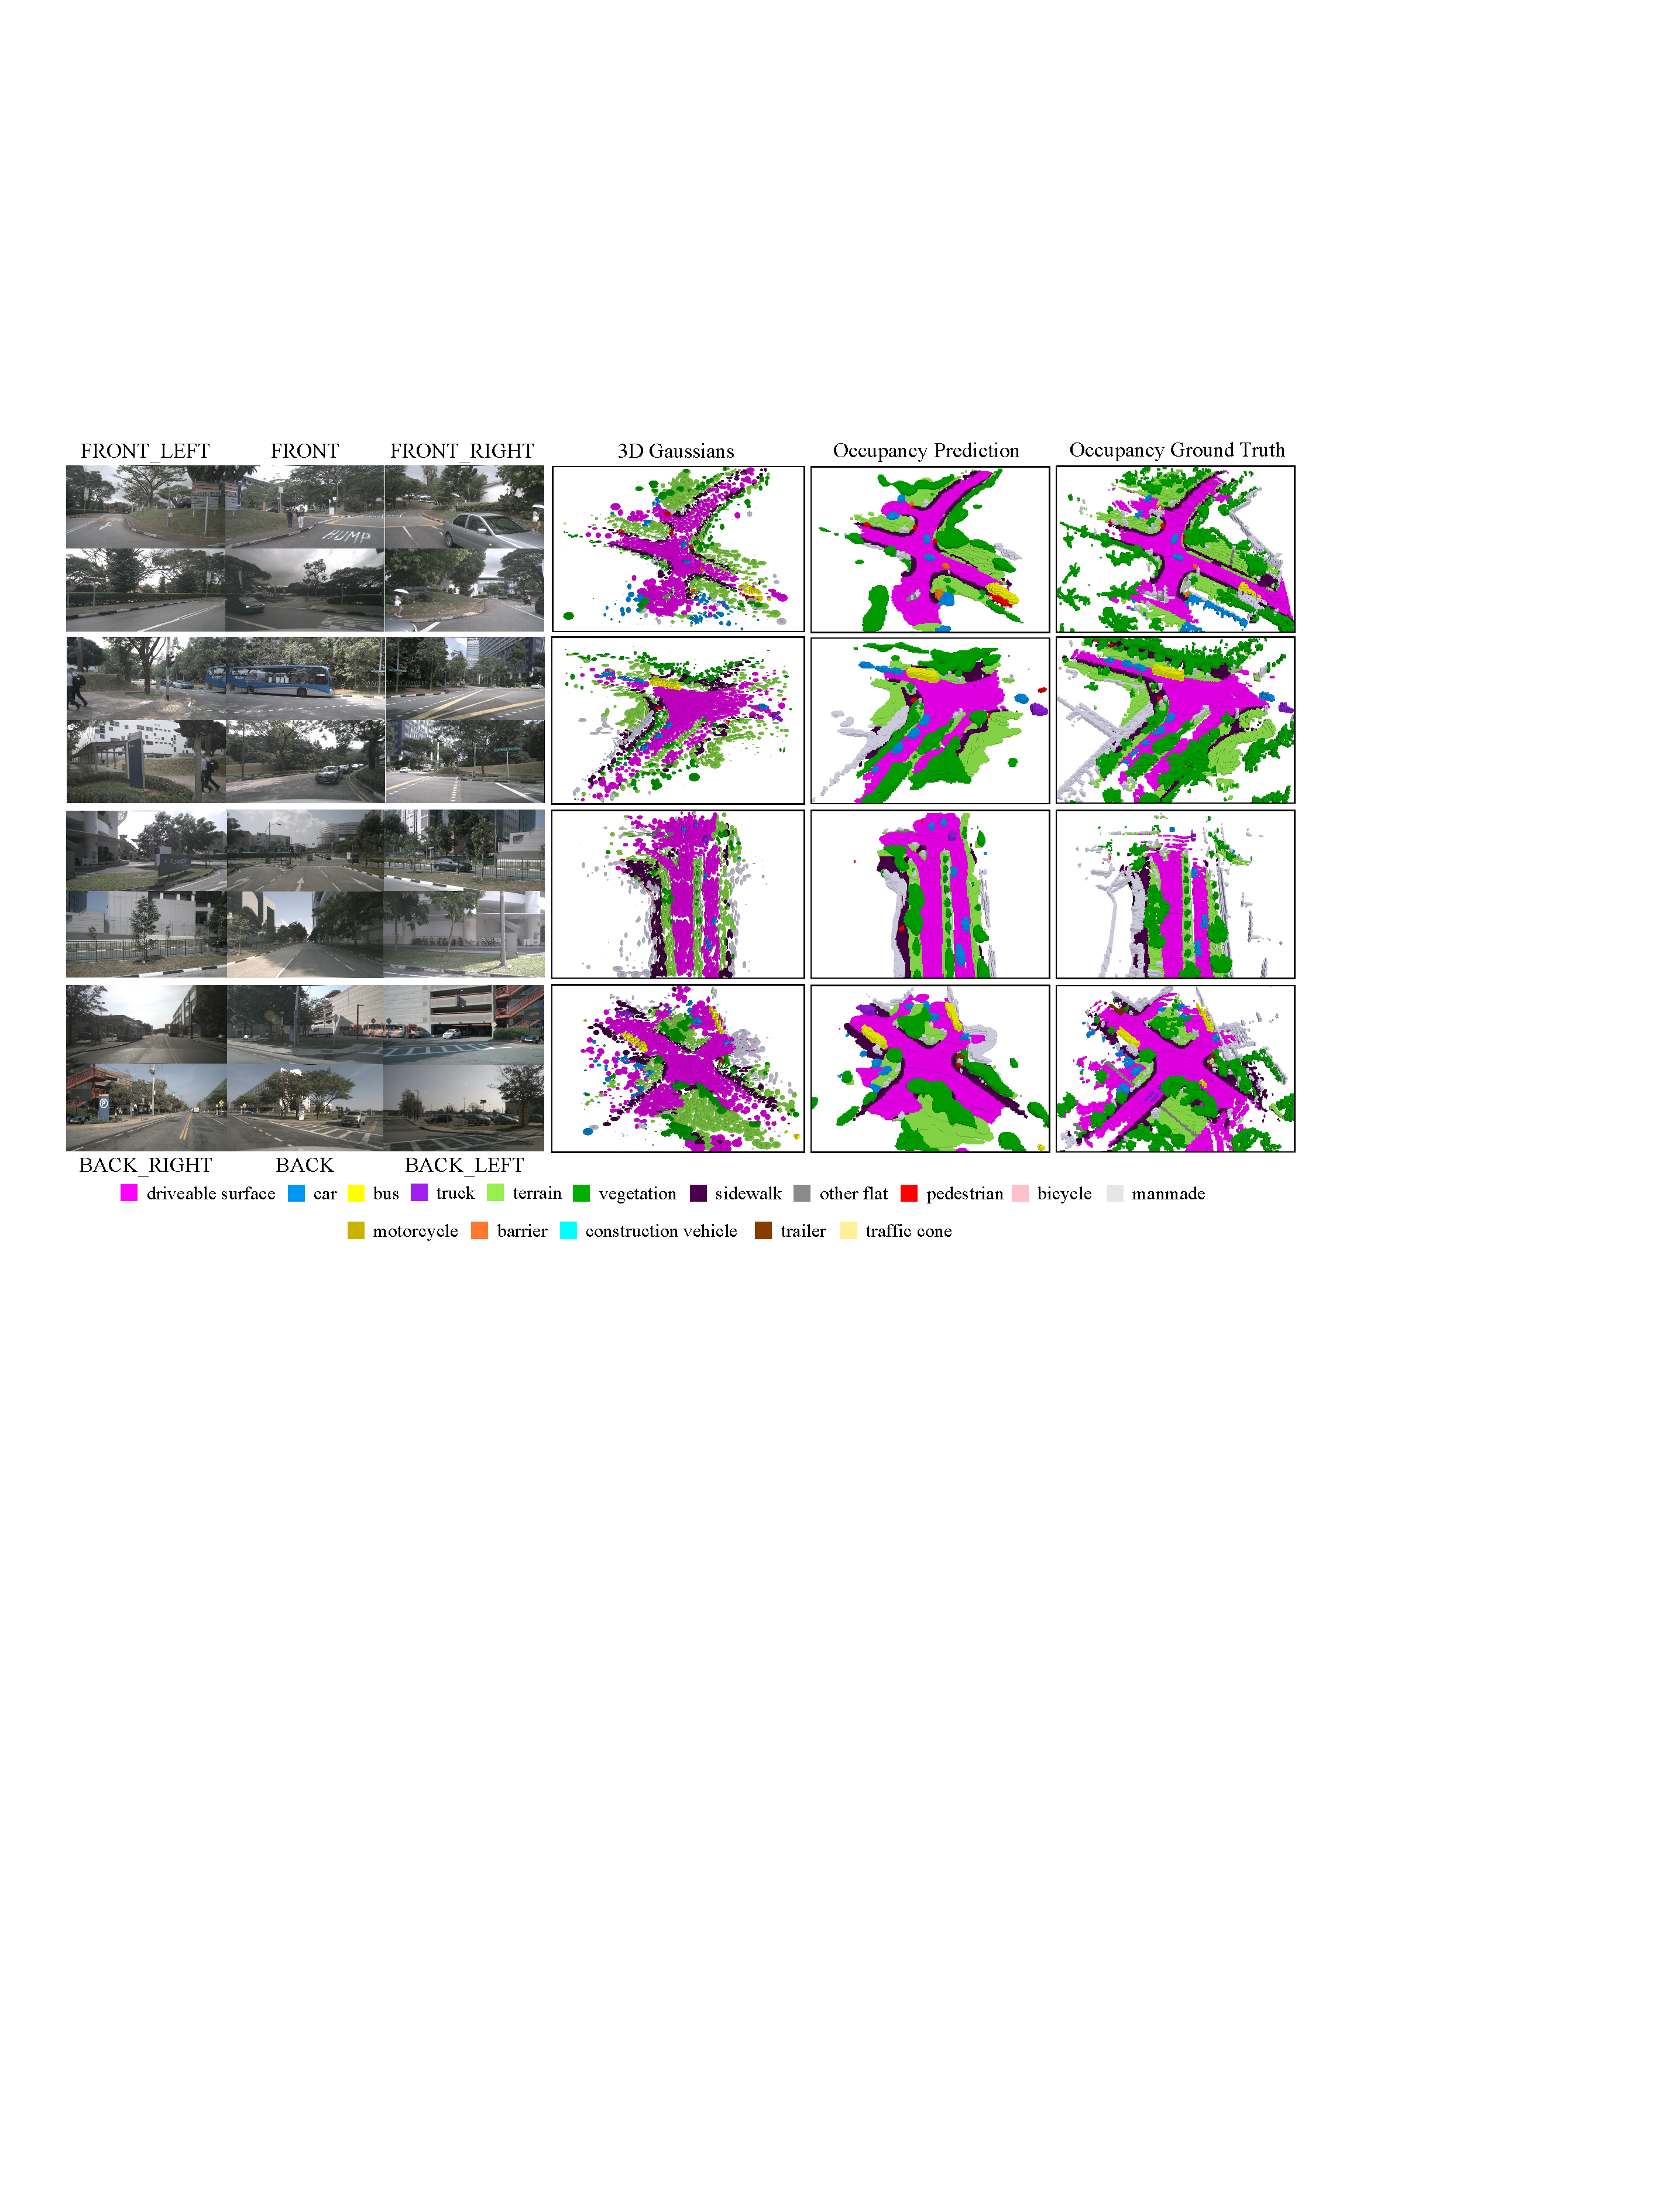
\includegraphics[width=0.95\linewidth]{figures/vis_main.pdf}
\vspace{-2mm}
\caption{\textbf{Gaussian and occupancy visualizations on nuScenes.}
Our model is able to predict both comprehensive and realistic 3D Gaussians and occupancy.
}
\label{fig:main}
\vspace{-6mm}
\end{figure*}



\begin{figure*}[t]
\centering
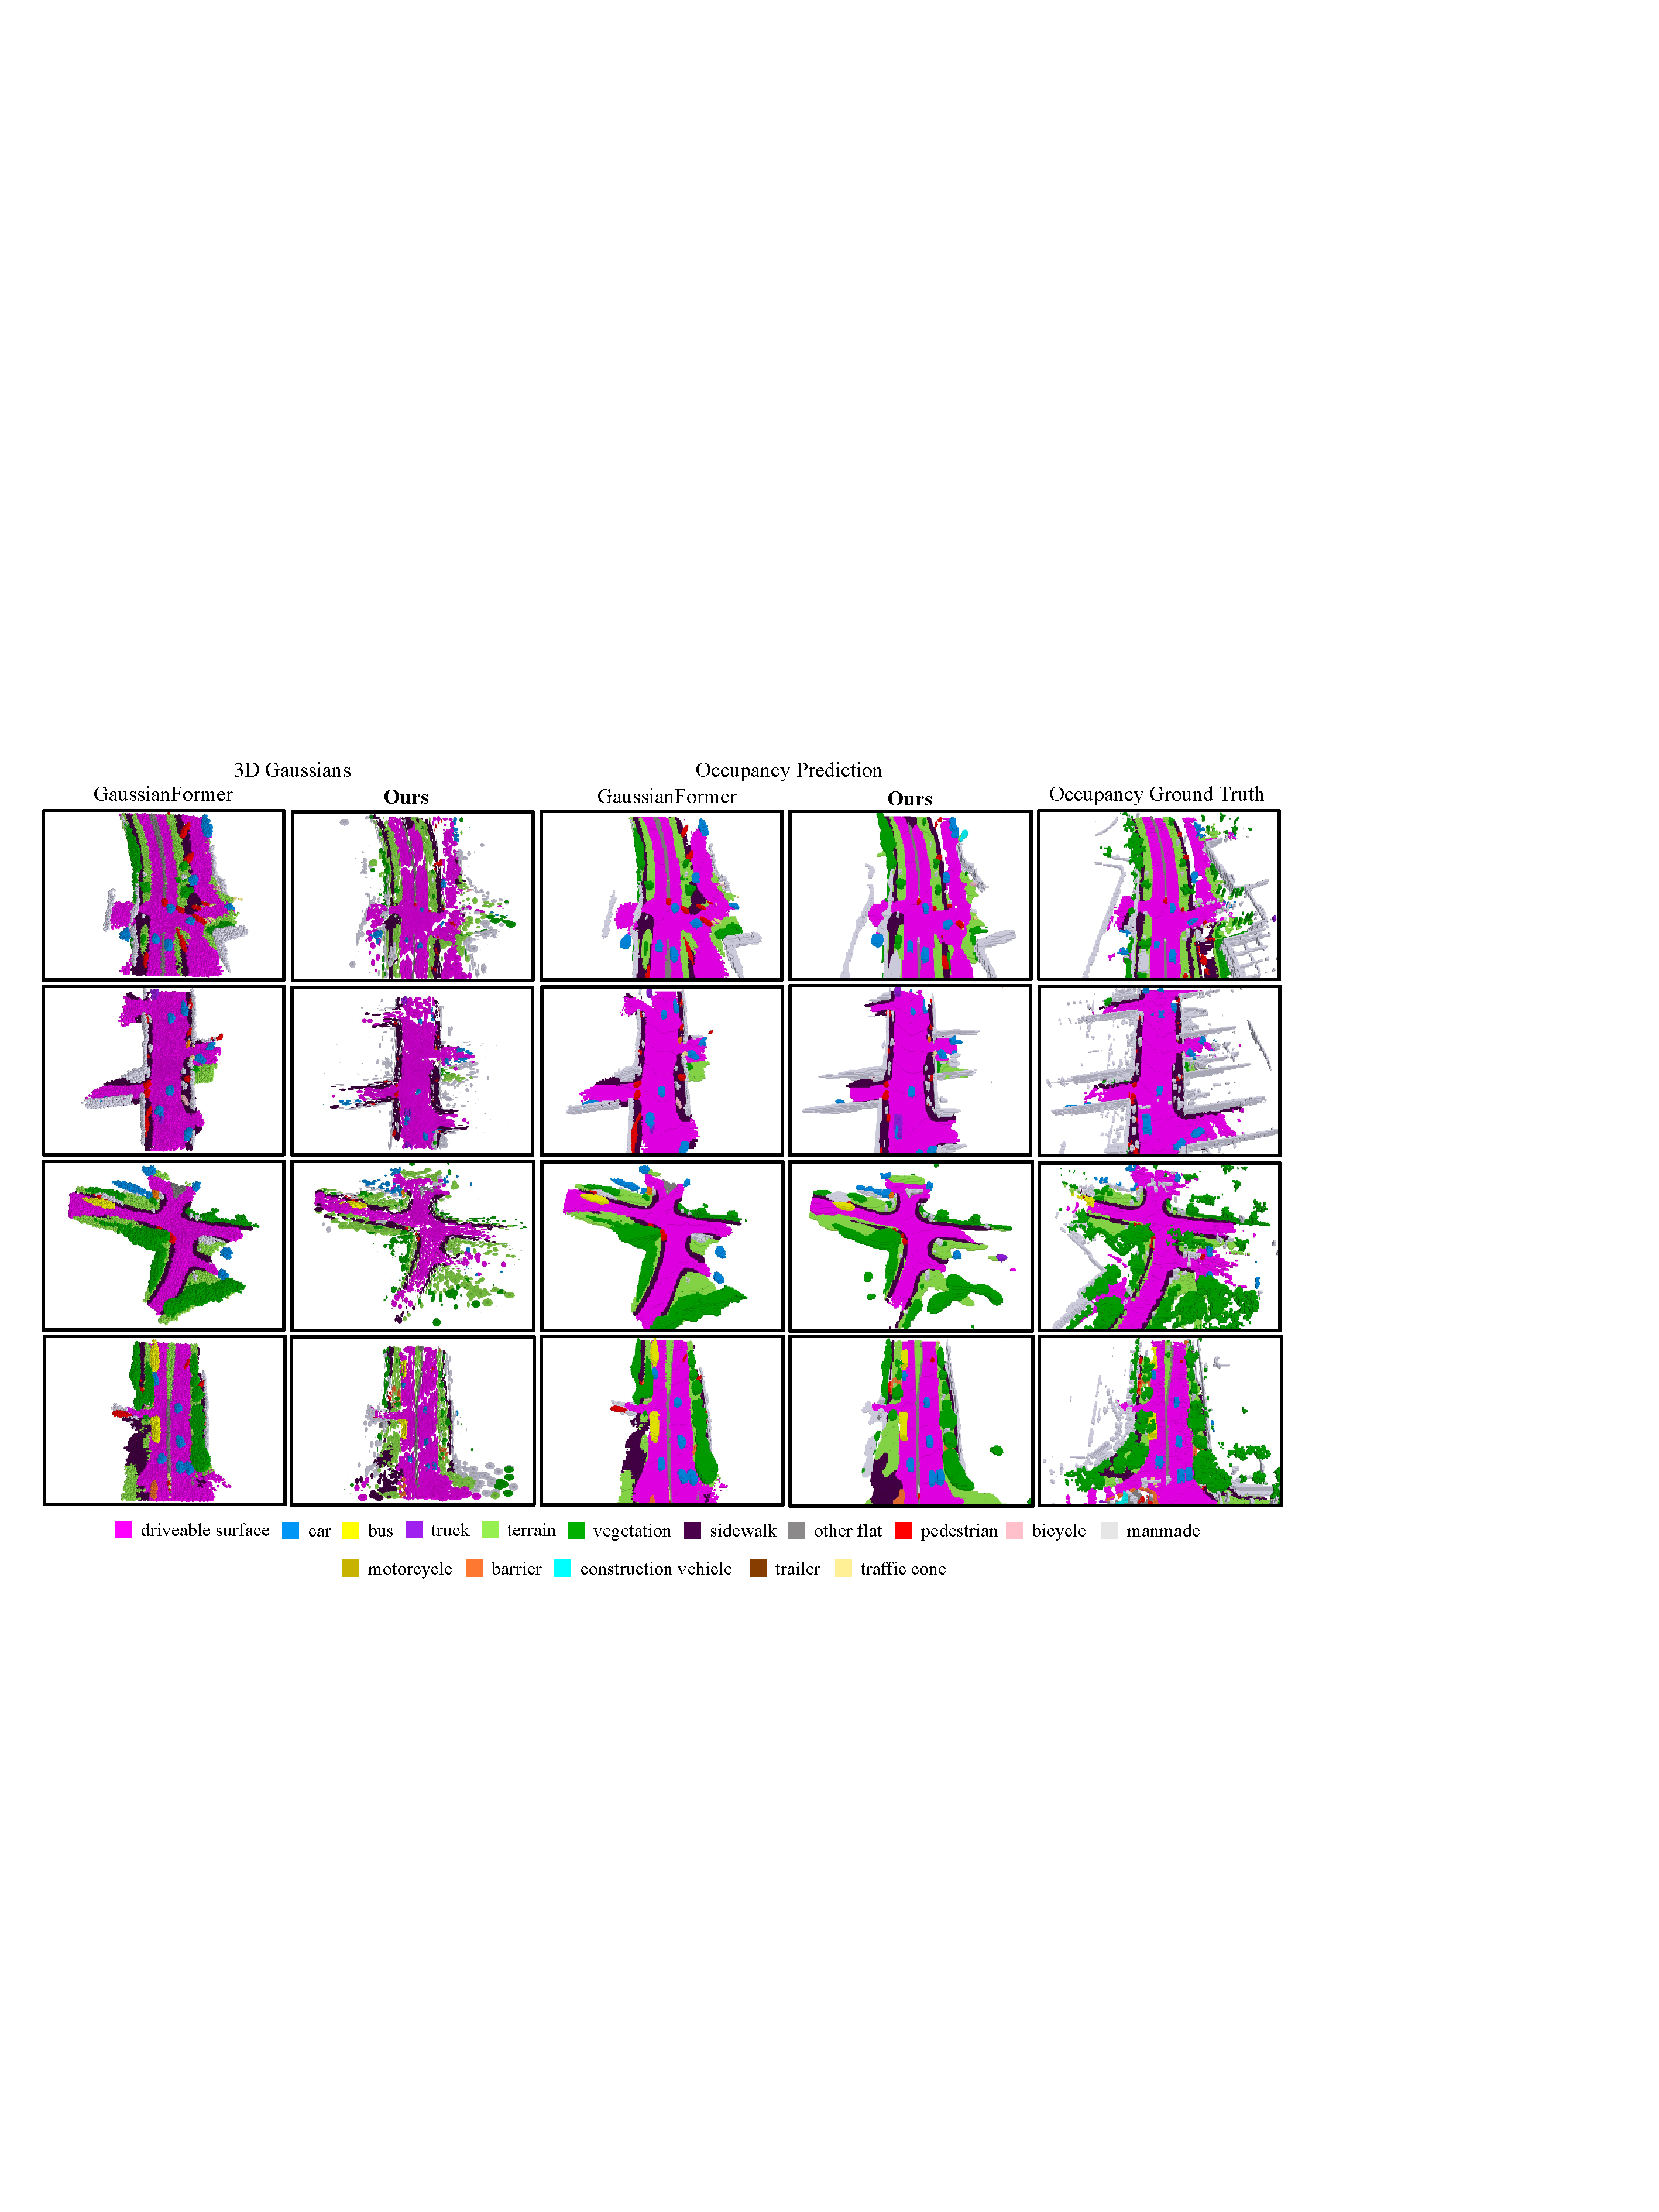
\includegraphics[width=0.95\linewidth]{figures/vis_comparison_1.pdf}
\vspace{-2mm}
\caption{\textbf{Comparison with GaussianFormer~\cite{huang2024gaussian}.}
Our method predicts 3D Gaussians with more adaptive shapes compared with GaussianFormer.
Although our method uses only 8.8\% Gaussians, it still generates comprehensive occupancy predictions and alleviates the elongated effect in GaussianFormer.
}
\label{fig:comparison}
\vspace{-3mm}
\end{figure*}


\begin{figure*}[!ht]
\centering
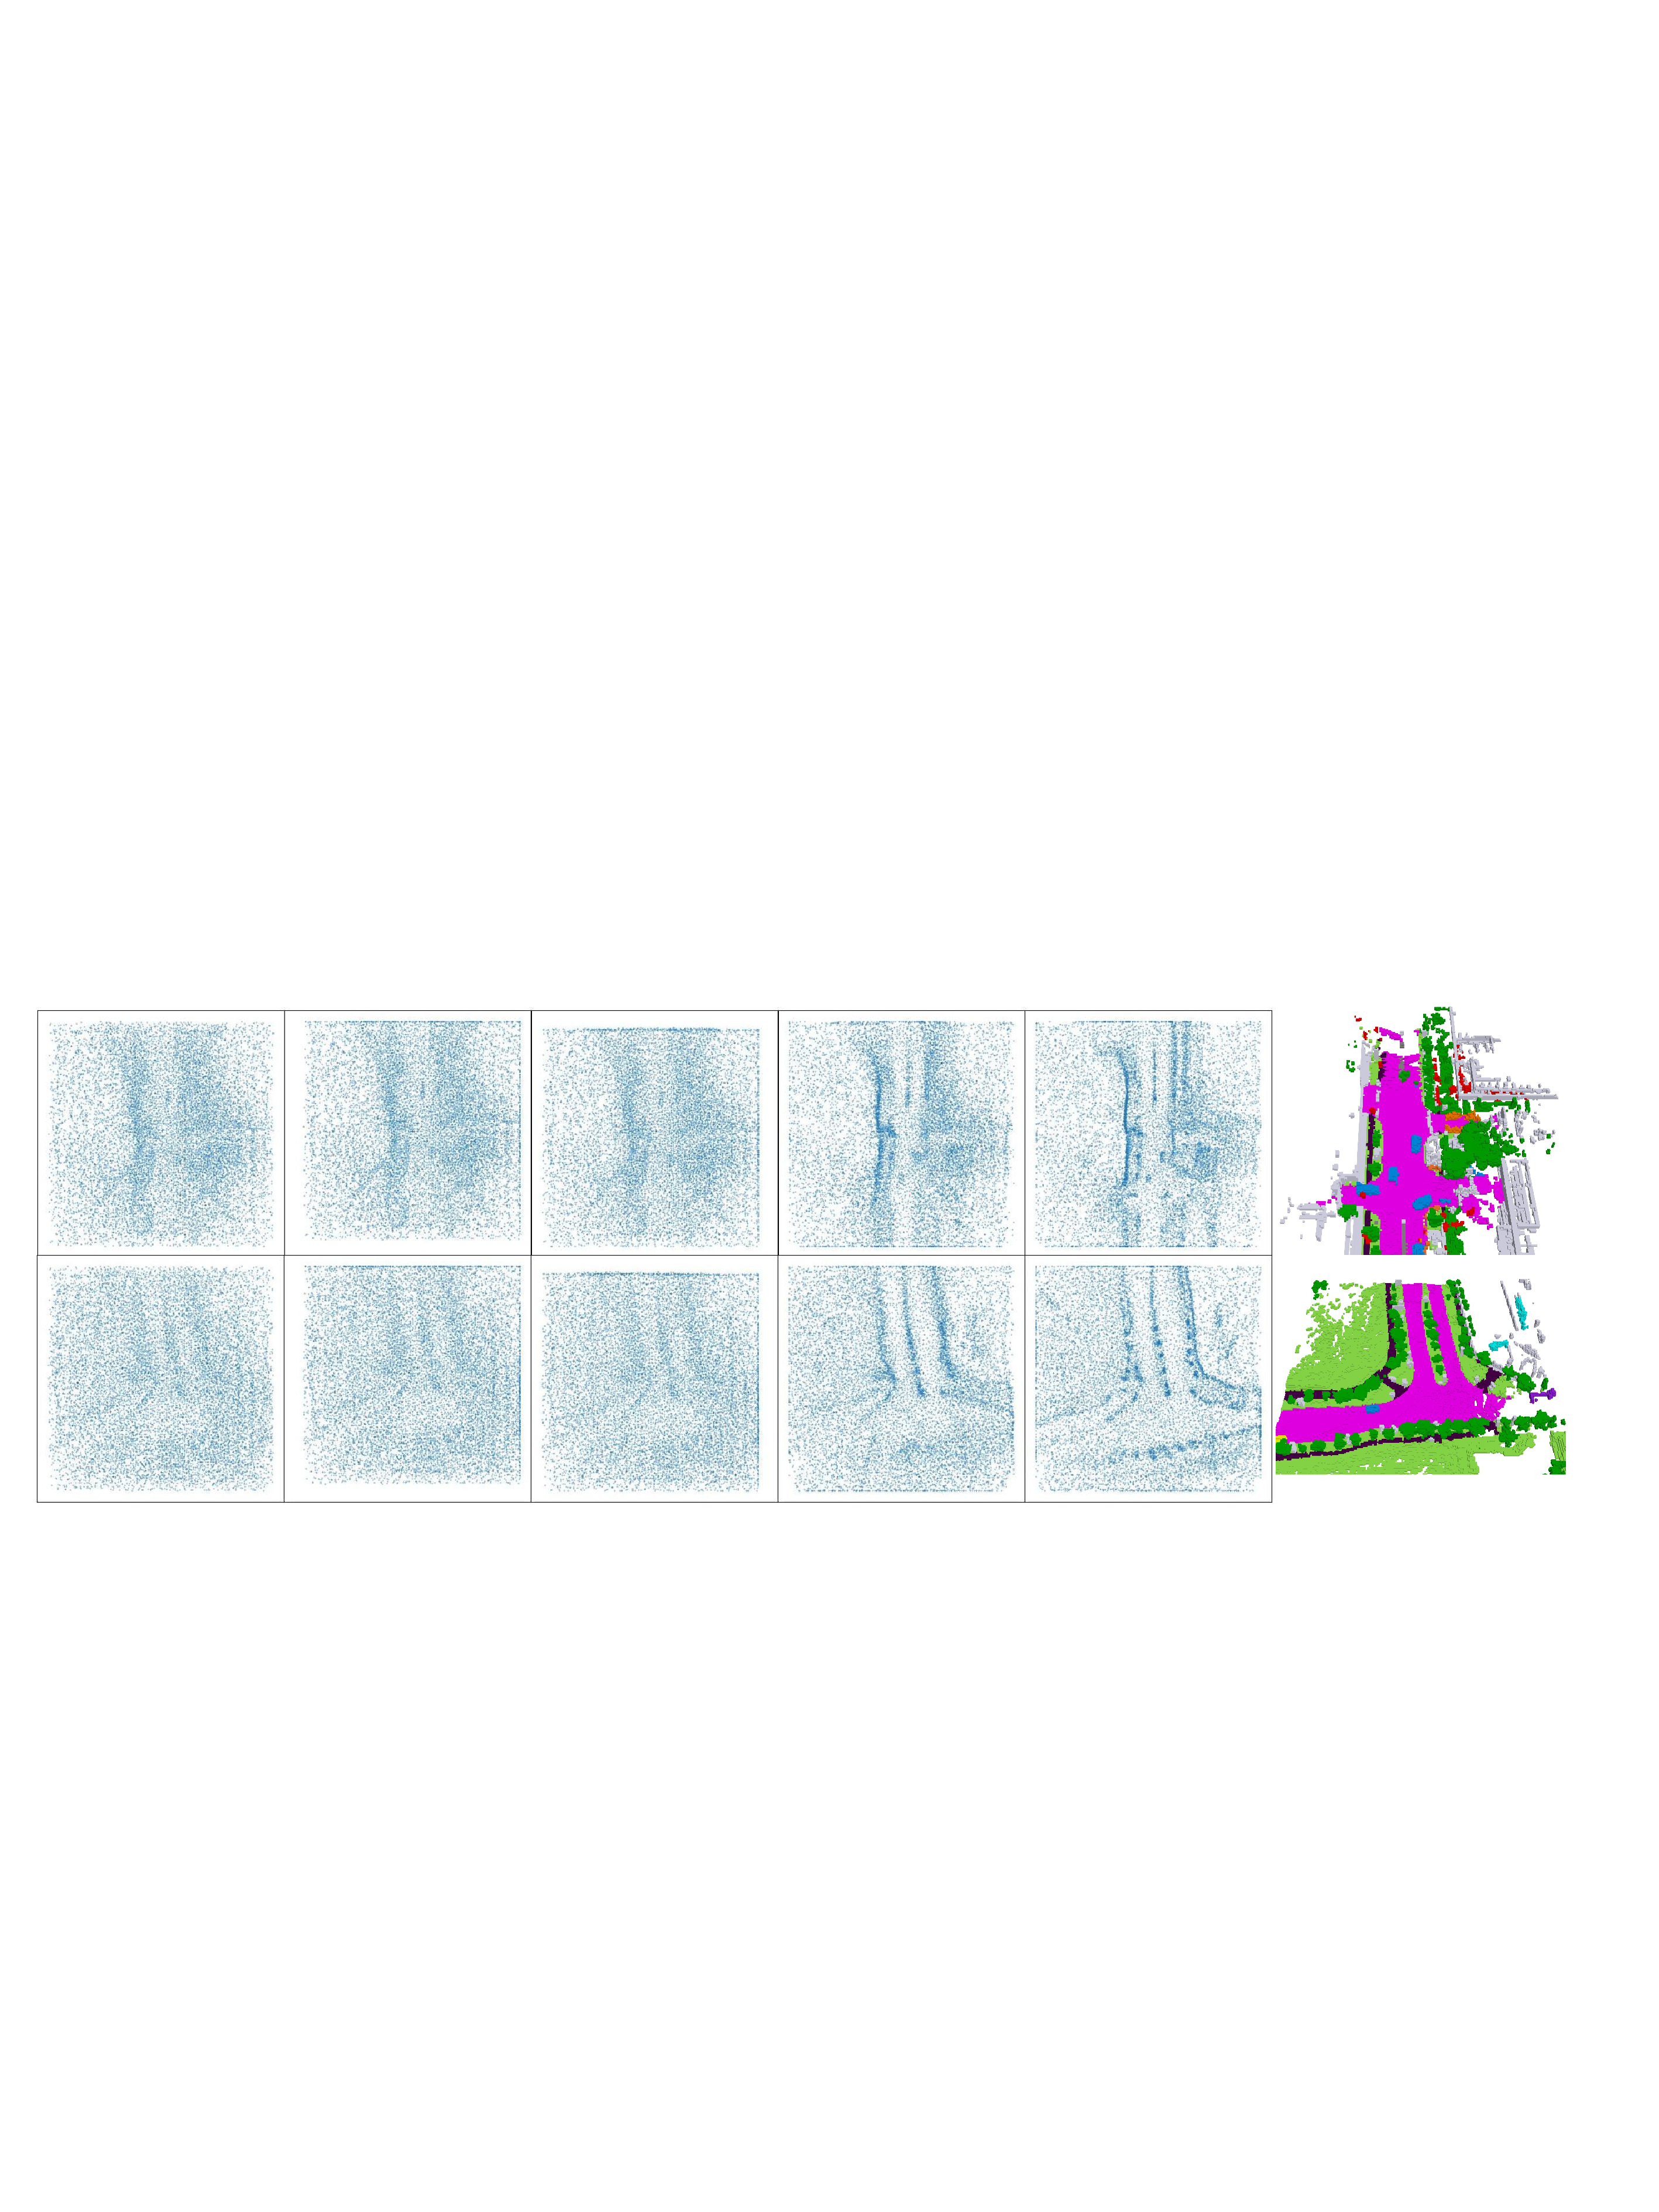
\includegraphics[width=0.95\textwidth]{figures/vis_moving.pdf}
\vspace{-2mm}
\caption{\textbf{Visualizations of Gaussian positions in the refinement process.}
We observe that our probabilistic Gaussians equipped with distribution-based intialization successfully learn to move towards occupied regions.
}
\label{fig:moving}
\vspace{-6mm}
\end{figure*}



\subsection{Ablation Study}


\textbf{Number of Gaussians.}
We report the influence of the number of Gaussians on the efficiency and performance of our model in Table~\ref{tab:number of gaussians}.
Our model achieves better performance-efficiency trade-off compared with GaussianFormer, outperforming it with less than 5\% number of Gaussians.
The latency of our method is higher than GaussianFormer, which we attribute to the time-consuming farthest point sampling (FPS) operation in our initialization module. 
We adopt the divide-and-conquer strategy to conduct the FPS operation in a batched manner for acceleration, and report the latency of the initialization module in parentheses.

\textbf{Design Choices.}
We conduct ablation study on the design choices of GaussianFormer-2 in Table~\ref{tab:components}.
We observe consistent improvement for both probabilistic modeling and distribution-based initialization module which surpasses the depth-based counterpart with a clear margin.


\textbf{Utilization of Gaussians.}
We provide comparisons on the utilization of Gaussians between GaussianFormer~\cite{huang2024gaussian} and our method in Table~\ref{tab:efficiency} using two important factors that reflect the utilization of Gaussians, which are position and overlap. 
Percentage of Gaussians in correct positions (Perc.) is percentage of Gaussians with their mean positions in the occupied space.
Overall overlap is calculated as summation of volumes of all Gaussians at 90\% over the coverage volume of all Gaussians, while individual overlap is computed by the average of the summation of the Bhattacharyya coefficient of each Gaussian with any other Gaussians.
We provide detailed information about these factors in the appendix.
Our method outperforms GaussianFormer on all these metrics, demonstrating better utilization.


\begin{table}[t]
    \centering
    \caption{
    \textbf{Ablation on the efficiency of GaussianFormer-2.}
    We set the number of Gaussians to 25600.
    Perc. and Dist. denote the percentage of Gaussians in correct positions, and the average distance of each Gaussian to its nearest occupied voxel, respectively.
    Overall and Indiv. represent the overall and individual overlapping ratios of Gaussians, respectively.
    }
    \vspace{-2mm}
    \setlength{\tabcolsep}{0.01\linewidth}
    \resizebox{1\linewidth}{!}{
    \begin{tabular}{c|cc|cc|cc}
        \toprule
        \multirow{2}{*}{Method} & \multicolumn{2}{c|}{Position} & \multicolumn{2}{c|}{Overlap} & \multirow{2}{*}{mIoU}   & \multirow{2}{*}{IoU} \\
        & Perc. (\%) \( \uparrow \) & Dist. (m) \( \downarrow \) & Overall \( \downarrow \) & Indiv. \( \downarrow \) \\
        \midrule
        GaussianFormer~\cite{huang2024gaussian} & 16.41 & 3.07 & 10.99 & 68.43 & 16.00 & 28.72   \\
        {Ours} & \textbf{28.85} & \textbf{1.24} & \textbf{3.91} & \textbf{12.48} & \textbf{20.32} & \textbf{31.04} \\
        \bottomrule
    \end{tabular}}
    \vspace{-7mm}
    \label{tab:efficiency}
\end{table}


\subsection{Visualizations}
We provide Gaussian and occupancy visualizations in Figure~\ref{fig:main}. 
Our model is able to predict reasonable Gaussian distributions and comprehensive occupancy results.
Further, we compare our method against GaussianFormer in Figure~\ref{fig:comparison}.
Our Gaussians are more adaptive in shape compared with isotropic spherical Gaussians in GaussianFormer.
We also visualize the xy coordinates of Gaussians in the initialization and subsequent blocks of GaussianFormer-2 in Figure~\ref{fig:moving}.
We find that the Gaussians successfully learn to move towards occupied area thanks to the object-centric probabilistic design and effective initialization module.


